\chapter{Sensitivity to dark matter signals}\label{cha:darkmatter}

The main goal of the thesis is to investigate if certain dark matter signals can be detected after the high luminosity upgrade. One immediate worry is that the background may become large in comparison to the signal, making the signal undetectable.

Another goal is to investigate if it might become more difficult to differentiate between the signal and background due to the degradation of jet and missing energy resolutions in the high luminosity upgrade.

This thesis focuses on using a luminosity of 1000 fb$^{-1}$ and a center of mass energy of 14 TeV. The reconstructed data is created using a pile-up rate $\obs{\mu} = 140$, as expected during phase II.

The signal models are given in \appendixref{sec:appsignals} along with the background models. The two classes of models were introduced in \subsectionref{sec:tb:subsec:eft} and will be discussed in more detail in this chapter.

Each signal model has been evaluated in different signal regions and the detectability has been evaluated using a statistical $p$-value. 

\newpage
\section{Signal over background}
\subsection{Signal Region}
An event is a recorded proton-proton collision which consists of hundreds or thousands of observables such as the number of electrons, muons, jets, tau leptons, gammas or E$^{Miss}_T$, each with their energy and momenta.

A signal region (\abbrSR) is defined as a set of selections on event variables designed to create a sample which is enriched in signal and depleted of background. One usually tries to design the signal region so that the signal is large enough and the background small enough that one would statistically be able to either:
\begin{itemize}
\item Exclude the signal if the observation of the data is compatible with a background only hypothesis.
\item Detect the signal and quantify the significance of the excess in data over background if the data is consistent with a signal plus background hypothesis.
\end{itemize}

How to define an optimal signal region is not known a priori and has to be studied for different signal models. The optimal region typically changes e.g. with a change of the mass of new particles, for instance the \abbrWIMP mass, or the suppression scale. This is why there are several different signal regions studied in this thesis.

\subsection{Cross section and luminosity weighting}
Each signal or background sample is simulated at a given luminosity. These luminosities are lower than $1000$fb$^{-1}$ which is of interest in this thesis. 

A weight is used to normalize different types of data so that they can be compared. 
As given in \eqref{eq:Numevents}, the total number of events can be estimated as:
\begin{equation*}
N=\sigma \int \mathscr{L} dt \equiv \sigma \Lagr
\end{equation*}
Thus if the samples are generated at different luminosities the following weight should be used to rescale the samples to a new luminosity:
\begin{equation}
weight=\frac{\Lagr \sigma}{N_{Raw}}
\end{equation}
where $N_{Raw}$ is the number of simulated events for a physical process, $\Lagr$ is the luminosity at which the samples are compared, and $\sigma$ is the cross-section. 

Since each process has its own cross-section it has its own weight which is larger than one, since the simulated luminosity is lower than 1000fb$^{-1}$.
In this thesis $\Lagr=10$fb$^{-1}$ is used to validate the background and $\Lagr=1000$fb$^{-1}$ when comparing the signals to the background.


\subsection{Background processes}
To emulate the background in a proton-proton collision simulations of the main processes, which are given in \tableref{tab:backproc2}, are used. 
\begin{table}[ht]
\begin{tabular}{|l|}
\hline
Process \\ \hline
Z$\rightarrow \nu \nu$ \\
W$\rightarrow e\nu$ \\
W$\rightarrow \mu \nu$ \\
W$\rightarrow \tau \nu$ \\ \hline
\end{tabular}
\caption{The main background processes from a collision. Each sample is a simulation of a physical process, the simulation names can be found in \appendixref{1backpro}.}
\label{tab:backproc2}
\end{table}

\subsection{Verification of background normalisation}\label{sec:sig:subsec:veri} 	
To verify that the background samples are correctly normalised they are compared with Ref. \citep{ATLAS-CONF-2012-147} in which the center of mass energy is 8 TeV and the luminosity is 10 fb$^{-1}$. 

The cross sections at 8 TeV are about 4 times lower than cross sections at 14 TeV.
These cross-sections are calculated with MadGraph\citep{madgraph} for the signal samples and Sherpa \citep{sherpa} for the background samples, as given in \appendixref{cha:datasets}. 

The pre-selection criteria used in Ref. \citep{ATLAS-CONF-2012-147} are the following:
\begin{itemize}
\item Jet veto, require no more than 2 jets with $p_T > 30 GeV$ and $|\eta| < 4.5$.  \\ 
This is done to reduce the number of multi-jet events.
\item Lepton veto, no electron or muon. \\
These vetos are there to remove uninteresting $W \rightarrow e \nu$ and $W \rightarrow \mu \nu$ background events.
\item Leading jet with $|\eta| < 2.0$ and $\Delta \varphi (jet, E_T^{Miss})>0.5$ (second-leading jet).\\ 
This is done to further reduce the number of multi-jet events.
\end{itemize}
The following signal regions were used:
\begin{table}[h]
\renewcommand{\arraystretch}{1.2} %Change back
\begin{center}
\begin{tabular}{l l l l l l}
\hline
signal region & SR3p & SR4p \\ \hline
minimum leading jet p$_T$ (GeV) & 350 & 500 \\
minimum E$^{Miss}_T$ (GeV) & 350 & 500 \\ \hline
\end{tabular}
\label{tab:oldsr}
\caption{The signal regions from Ref. \citep{ATLAS-CONF-2012-147}.}
\end{center}
\renewcommand{\arraystretch}{1.0} %Change back
\end{table}

The article in Ref. \citep{ATLAS-CONF-2012-147} has four signal regions in total, unfortunately since the simulated background used in this thesis is filtered before the analysis only the two highest regions are comparable. This can be seen in \tableref{tab:Compare1} in \subsectionref{Verifying background data}.

The background is compared to Ref. \citep{ATLAS-CONF-2012-147} altering the cross-sections of the samples used in this thesis to simulate a center of mass energy of 8 TeV instead of 14. This could unfortunately not be done for the signals as that would require new samples to be produced. As seen in \tableref{tab:Compare1} and somewhat discussed in \subsectionref{Verifying background data} the events corresponded quite nicely to the values from the paper. The discrepancies are explained by general differences between simulations and measured events, such as:
\begin{itemize}
\item The difference in W$\rightarrow\tau\nu$ can be explained by the fact that $\tau$ can not be recreated as a jet in the simulated events which it can in measured events.

\item The difference in W$\rightarrow\mu\nu$ is explained through the simulated events having a better separation of muon neutrinos and E$_T^{Miss}$.
\end{itemize}

\subsection{Errors in background}\label{subsec:errdata}
To make a thorough analysis of the background it is important to take into consideration different errors that exist in the predicted number of events. This is especially important when looking at which signals can be excluded in different signal regions, since a large uncertainty on the background has a negative impact on the sensitivity to the signal.



The uncertainties are divided into three categories:
\begin{itemize}
\item Uncertainty due to limited Monte Carlo (\abbrMC) statistics. \\
The statistical errors from \abbrMC come from the number of events that are generated for a certain process and can not be estimated since it is not known how many events which will be simulated in the future.

\item Uncertainty due to limited statistics in data control regions.\\
A control region (\abbrCR) is the opposite to a signal region,  criteria set so that there is a region with almost no signal. In this \abbrCR there will still be fluctuations in the amount of background events due to statistical effects, which can then be measured. The numerical value, whose size is a priori constant with the luminosity, has been take from Ref. \citep{ATLAS-CONF-2012-147} as $\frac{30}{380}$ and is assumed to decrease with the increased luminosity as $\frac{1}{\sqrt{\Lagr}}$.

\item Other systematic errors.\\
The systematic errors are fixed errors which are always present coming from different approximations in how all the events are generated. The other systematic errors have been given two different values, from Ref. \citep{ATLAS-CONF-2012-147} as $\frac{30}{380}$ or 0.02.
\end{itemize}

Using the errors above results in two different models of the total error in the background $\sigma_B$ which is defined as:
\begin{equation*}
\sigma_B = \text{Statistical error from \abbrMC} \oplus \text{Statistical error in \abbrCR} \oplus \text{Other errors}
\end{equation*}
Numerically the total error being used is 0.08 or 0.02. 

\subsection{Figure of merit}\label{subsec:figmer}
To be able to evaluate different signal regions and different signal models, a figure of merit $p$ is used. The value $p$ is the probability for the observed background to fluctuate to the value of the signal plus background. Thus if the $p$-value is small it is improbable that the observed background could result in the same value as if there is a signal and background. This means that for a sufficiently small $p$-value the signal is detectable. The limiting value in this thesis is taken as $p=0.05$, everything below is considered detectable. 

Assuming that the expected number of background events are $B \pm \sigma_B$ where $\sigma_B$ is the quadratic sum of the errors as explained in \subsectionref{subsec:errdata}. The expected number of signal events is $S$, not to be confused with the variable $S$ in \sectionref{sec:smear}, assumed without fluctuation. 

If no uncertainty in $B$ or $S$ is assumed, then the probability that the background will fluctuate up to the signal and background should follow a Poisson distribution as such:
\begin{equation}
\text{P($S$+$B$|$B$)}=\frac{e^{-B}B^{(S+B)}}{(S+B)!}
\end{equation} 

The probability that the observed number of background events $O$ will fluctuate to a value larger than or equal to the signal plus background then becomes:
\begin{equation}
\text{P($O$$ \geq$$S$+$B$|$B$)} =\sum_{k=S+B}^{\infty}  \frac{e^{-B}B^k}{k!}
\end{equation} 

However, since there is an uncertainty in the background, the probability distribution P(O$ \geq$S+B|B) must be weighted with a Gaussian function:
\begin{equation}
 \text{G($N_B$|$B$,$\sigma_B$)}=\frac{1}{\sigma_B \sqrt{2 \pi}} e^{-\frac{(N_B-B)^2}{2\sigma_B^2}}
\end{equation}
where $N_B$ is the expected number of background events. 

The probability of the background fluctuating to signal plus background is calculated as:
\begin{equation}
p = \int\limits_{-\infty}^{\infty} \text{P($O$$ \geq$$S$+$B$|$N_B$)G($N_B$|$B$,$\sigma_B$)} dN_B
\end{equation}

\subsection{D5 operator models}\label{sec:signal:subsec:d5}
As described in \subsectionref{sec:tb:subsec:eft}, one of the signals is modelled using the D5 operator. In this thesis two different scenarios are used, one at a dark matter mass of 50 GeV and one at 400 GeV. The different datasets for the signals are presented in \tableref{tab:d5data} in \appendixref{d5pro}.

Each of these models is modelled with a mass suppression scale, denoted $M$*, at 10000 GeV which is connected to the cross-section as shown in \eqref{eq:sigmas}. To study another $M$* the cross section has to be altered by using:
\begin{equation}\label{eq:sigmas}
\sigma \text{($M$*)} = \frac{\sigma_{reference}}{\text{$M$*}} 
\end{equation}
where $\sigma_{reference}$ is the theoretically calculated sigma.
In \subsectionref{sec:res:subsec:m*} it is determined which values of $M$* can be excluded with the upgraded \abbrLHC phase II upgrade and \abbrATLAS .

\subsection{Light vector mediator models}\label{sec:signal:subsec:vecmed}
As described in \subsectionref{sec:tb:subsec:eft}, the other signal model is a vector mediator model. In this thesis these signals have two different width scenarios, $M$/3 and $M$/8$\pi$ where $M$ denotes the mediator mass. The width scenarios contain eight different mediator mass scenarios with masses between 100 and 15000 GeV. In addition to this there are, as with the D5 operator, two different dark matter masses, one at 50 GeV and one at 400 GeV. The different datasets are presented in \tableref{tab:vecmeddata} in \appendixref{livecmedpro}.

The models found to be excludable are presented in \subsectionref{sec:res:subsec:Mm}. 
\newpage
\section{Signal regions}
\subsection{Signal region definitions}\label{sec:sr:subsec:srd}
To be able to compare signal results to previous studies new signal regions were devised. When simulated only 2 \% of the estimated signal events passed the pre-selection criteria compared to estimations. Thus these new pre-selection criteria were devised to increase the amount of signal. 

The following pre-selection criteria are used:
\begin{itemize}
\item Jet veto, require no more than 2 jets with $p_T > 30 GeV$ and $|\eta| < 4.5$.  \\ 
This is done to reduce the number of multi-jet events.
\item Electron veto which is defined: $\Delta R (jet^{lead},electron^{lead})\geq 0.4$ and \\
$electron^{lead} p_T>20 GeV$ removed.
\item Muon veto which is defined: $\Delta R (jet^{lead},muon^{lead})\geq 0.4$ and \\
$muon^{lead} p_T>20 GeV$ removed. \\
These formulation of vetos are used to remove uninteresting $W \rightarrow e \nu$ and $W \rightarrow \mu \nu$ background events without removing too much of the signal. The $\Delta R$ involvement is to make sure that the veto is only on simulated true particles and not simulated false detections.
\item Leading jet with $|\eta| < 2.0$ and $\Delta \varphi (jet, E_T^{Miss})>0.5$ (second-leading jet).\\ 
This is done to further reduce the number of multi-jet events.
\end{itemize}
Here the superscript lead denotes the entity with highest transverse momentum $p_T$. Thus $electron^{lead}$ would be the simulated electron in an event with the highest $p_T$.

To try and minimize the amount of background compared to the amount of signal, the following  signal regions are used:
\begin{table}[h]
\renewcommand{\arraystretch}{1.2} %Change back
\begin{center}
\begin{tabular}{l l l l l l}
\hline
Symmetric signal region & SR1 & SR1p & SR2 & SR3 & SR4 \\ \hline
minimum leading jet p$_T$ (GeV) & 350 &500& 600 & 800 & 1000 \\
minimum E$^{Miss}_T$ (GeV) & 350&500 & 600 & 800 & 1000 \\
\end{tabular}
\begin{tabular}{l l l l l} \hline
Asymmetric signal region & SRa &  SRb & SRc & SRd \\ \hline
minimum leading jet p$_T$ (GeV) & 350 & 350 & 350 & 350 \\
minimum E$^{Miss}_T$ (GeV) & 350 & 600 & 800 & 1000 \\ \hline
\end{tabular}
\caption{The new signal regions.}
\label{tab:newsr}
\end{center}
\renewcommand{\arraystretch}{1.0} %Change back
\end{table}

Where symmetric and asymmetric denote if criteria are the same or different for $p_T$  and  $E^{Miss}_T$.
These regions are constructed to be similar to previous studies and by looking at the distribution of leading jet $p_T$  and  $E^{Miss}_T$ for the signal and background samples. 
\subsection{Verifying background data}
The choice of a new electron and muon veto require the comparison from \subsectionref{sec:sig:subsec:veri} to be redone. As seen in \tableref{tab:newcomp} the events corresponded quite nicely to the values from the paper and are somewhat better than the previous comparison which can be seen in \subsectionref{Verifying background data}.

\newpage
\section{Results}\label{chap:sig:sec:res}
\subsection{Verifying background data}\label{Verifying background data}
In \tableref{tab:Compare1} and \tableref{tab:newcomp} a comparison is shown between the number of events in this work using 8 TeV center of mass energy cross section for 1000 fb$^{-1}$ at a truth level and the number of expected events predicted in Ref. \citep{ATLAS-CONF-2012-147} scaled to 1000 fb$^{-1}$. Truth data was used to not let the increased pile-up value affect the comparison. It can be seen that the simulated events and expected events coincide well for all processes and all regions apart from W$\rightarrow\tau\nu$, W$\rightarrow\mu\nu$ and thus the total as well. 

\begin{table}[ht]
\begin{center}
\begin{tabular}{|l|l|l|l|l|}
\hline
& \multicolumn{2}{c}{SR3p} & \multicolumn{2}{|c|}{SR4p} \\
\hline
Process & Simulated & From paper & Simulated & From paper \\ \hline
Z$\rightarrow\nu\nu$ & 140298 & 152000 & 25250 & 27000 \\
W$\rightarrow\tau\nu$ & 40701 & 37000 & 5862 & 3900 \\
W$\rightarrow e\nu$ & 11229 & 11200 & 1507 & 1600 \\
W$\rightarrow\mu\nu$ & 13727 & 15800 & 1872 & 4200 \\ \hline
Total background & 205955 & 218000 & 34491 & 36700 \\ \hline
\end{tabular}
\caption{Comparison of the simulated and expected events from Ref. \citep{ATLAS-CONF-2012-147} at $\Lagr=1000$fb$^{-1}$, cross-sections corresponding to $\sqrt{s}=8$TeV.}
\label{tab:Compare1}
\end{center}
\end{table}

\begin{table}[ht]
\begin{center}
\begin{tabular}{|l|l|l|l|l|}
\hline
& \multicolumn{2}{c}{SR1} & \multicolumn{2}{|c|}{SR1p} \\
\hline
Process & Simulated  & From paper & Simulated & From paper  \\ \hline
Z$\rightarrow\nu\nu$ & 150753 & 152000 & 27569 & 27000 \\
W$\rightarrow\tau\nu$ & 49320 & 37000 & 7318 & 3900 \\
W$\rightarrow e\nu$ & 18329 & 11200 & 2534 & 1600 \\
W$\rightarrow\mu\nu$ & 22290 & 15800 & 3218 & 4200 \\ \hline
Total background & 240690 & 218000 & 40639 & 36700 \\ \hline
\end{tabular}
\caption{Comparison of the simulated and expected events from Ref. \citep{ATLAS-CONF-2012-147} with $\Lagr=1000$fb$^{-1}$, cross-sections corresponding to $\sqrt{s}=8$TeV and using a modified electron and muon veto as discussed in \subsectionref{sec:sr:subsec:srd}.}
\label{tab:newcomp}
\end{center}
\end{table}


\subsection{Signal and background events in signal regions}
In the following tables the number of events are given using one of the D5 operators as the signal, and the background in the different signal regions at $\sqrt{s}=14$ TeV and $\Lagr=1000$fb$^{-1}$. The number of background events is used to calculated exclusion limits on $M$* and on the mediator mass models.

%\renewcommand{\arraystretch}{1.0} %Change back
%\renewcommand{\arraystretch}{1.5} %Change height of tabel
\begin{landscape}
\begin{table}[ht]
\begin{center}
\begin{tabular}{|l|l|l|l|l !{\vrule width 4pt} l|l|l|l|}
\hline
Process & SR1 & SR2 & SR3 & SR4 & SRa & SRb & SRc & SRd \\ \hline
D5, $m_{\chi}=50$ GeV, M*=1TeV & 131844 & 30900 & 11053 & 4532 & 131844 & 37217 & 13280 & 5387 \\ \hline
Z$\rightarrow\nu\nu$ & 619752 & 44146 & 8764 & 2205 & 619752 & 61193 & 11975 & 2998 \\
W$\rightarrow\tau\nu$ & 169983 & 8753 & 1479 & 344 & 169983 & 12047 & 2032 & 453\\ 
W$\rightarrow e\nu$ & 63026 & 2986 & 510 & 114 & 63026 & 4114 & 688 & 160 \\
W$\rightarrow\mu\nu$ & 76618 & 3880 & 658 & 162 & 76618 & 5094 & 871 & 199 \\ \hline
Total background & 929379 & 59765 & 11411 & 2825 & 929379 & 82448 & 15566 & 3810 \\ \hline
\end{tabular}
\caption{Signal and background events for truth data in the signal regions at $\sqrt{s}=14$ TeV and $\Lagr=1000$fb$^{-1}$.}
\label{tab:srtruth1}
\end{center}
\vspace*{5px}
\begin{center}
\begin{tabular}{|l|l|l|l|l !{\vrule width 4pt} l|l|l|l|}
\hline
Process at $\sqrt{s}=14$TeV& SR1 & SR2 & SR3 & SR4 & SRa & SRb & SRc & SRd \\ \hline
D5, $m_{\chi}=50$ GeV, M*=1TeV & 122117 & 28663 & 10273 & 4259 & 122117 & 39618 & 14151 & 5679 \\ \hline 
Z$\rightarrow\nu\nu$ & 568410 & 40518 & 8012 & 2023 & 568410 & 74564 & 13817 & 3318 \\
W$\rightarrow\tau\nu$ & 170999 & 8644 & 1442 & 314 & 170999 & 16241 & 2446 & 536 \\
W$\rightarrow e\nu$ & 60071 & 2799 & 470 & 110 & 60071 & 5366 & 835 & 183 \\
W$\rightarrow\mu\nu$ & 73495 & 3704 & 629 & 152 & 73495 & 6622 & 1046 & 236 \\ \hline
Total background & 872975 & 55665 & 10552 & 2599 & 872975 & 102793 & 18144 & 4273 \\ \hline 
\end{tabular}
\caption{Signal and background events for reconstructed data with $\obs{\mu}=140$ in the signal regions at $\sqrt{s}=14$ TeV and $\Lagr=1000$fb$^{-1}$.}
\label{tab:srreco1}
\end{center}
\end{table}
\end{landscape}

\Tableref{tab:srtruth1} and \tableref{tab:srreco1} show how the ratio between the number of signal events and total background increases from the first (SR1/SRa) to the last signal region (SR4/SRd) which illustrates that these are good choices of signal regions. The difference between SR4 and SRd show clearly the effect of the lead jet momenta cut. Comparing the two tables it is interesting to see that they are similar even though \tableref{tab:srreco1} is reconstructed with a pile-up rate of 140 which is consistent with a small effect of pile-up.
\subsection{Project exclusion limits on M*}\label{sec:res:subsec:m*}
For the D5 operators as described in \subsectionref{sec:signal:subsec:d5}, limits on the mass suppression scale has been calculated by calculating the $p$-value for each value of $M$* in the range 0 to 2500 GeV and finding which values of M* lead to $p<0.05$. This is done using the two different error models as described in \subsectionref{subsec:errdata} as figures of merit.

The limit is found, seen as a horizontal line in both \figureref{fig:SRnewMt} and \figureref{fig:SRnewMr}, when the $p$-value = 0.05. In these figures the effect of the error model can be seen as a left shift but no change in incline. The $p$-value is low at low $M$* since the cross-section is large which leads to a large signal which is easy to exclude. Higher values of $M$* decrease the value of the cross-section making it more difficult and finally improbable to distinguish the signal from the background. For example a $p$-value of 0.5 indicated that the observed value of the background has a 50 \% chance to fluctuate to the value of signal plus background.

 \begin{figure}[H] %!ht
    \subfloat[ \label{fig:SRnewMt:1}]{%
     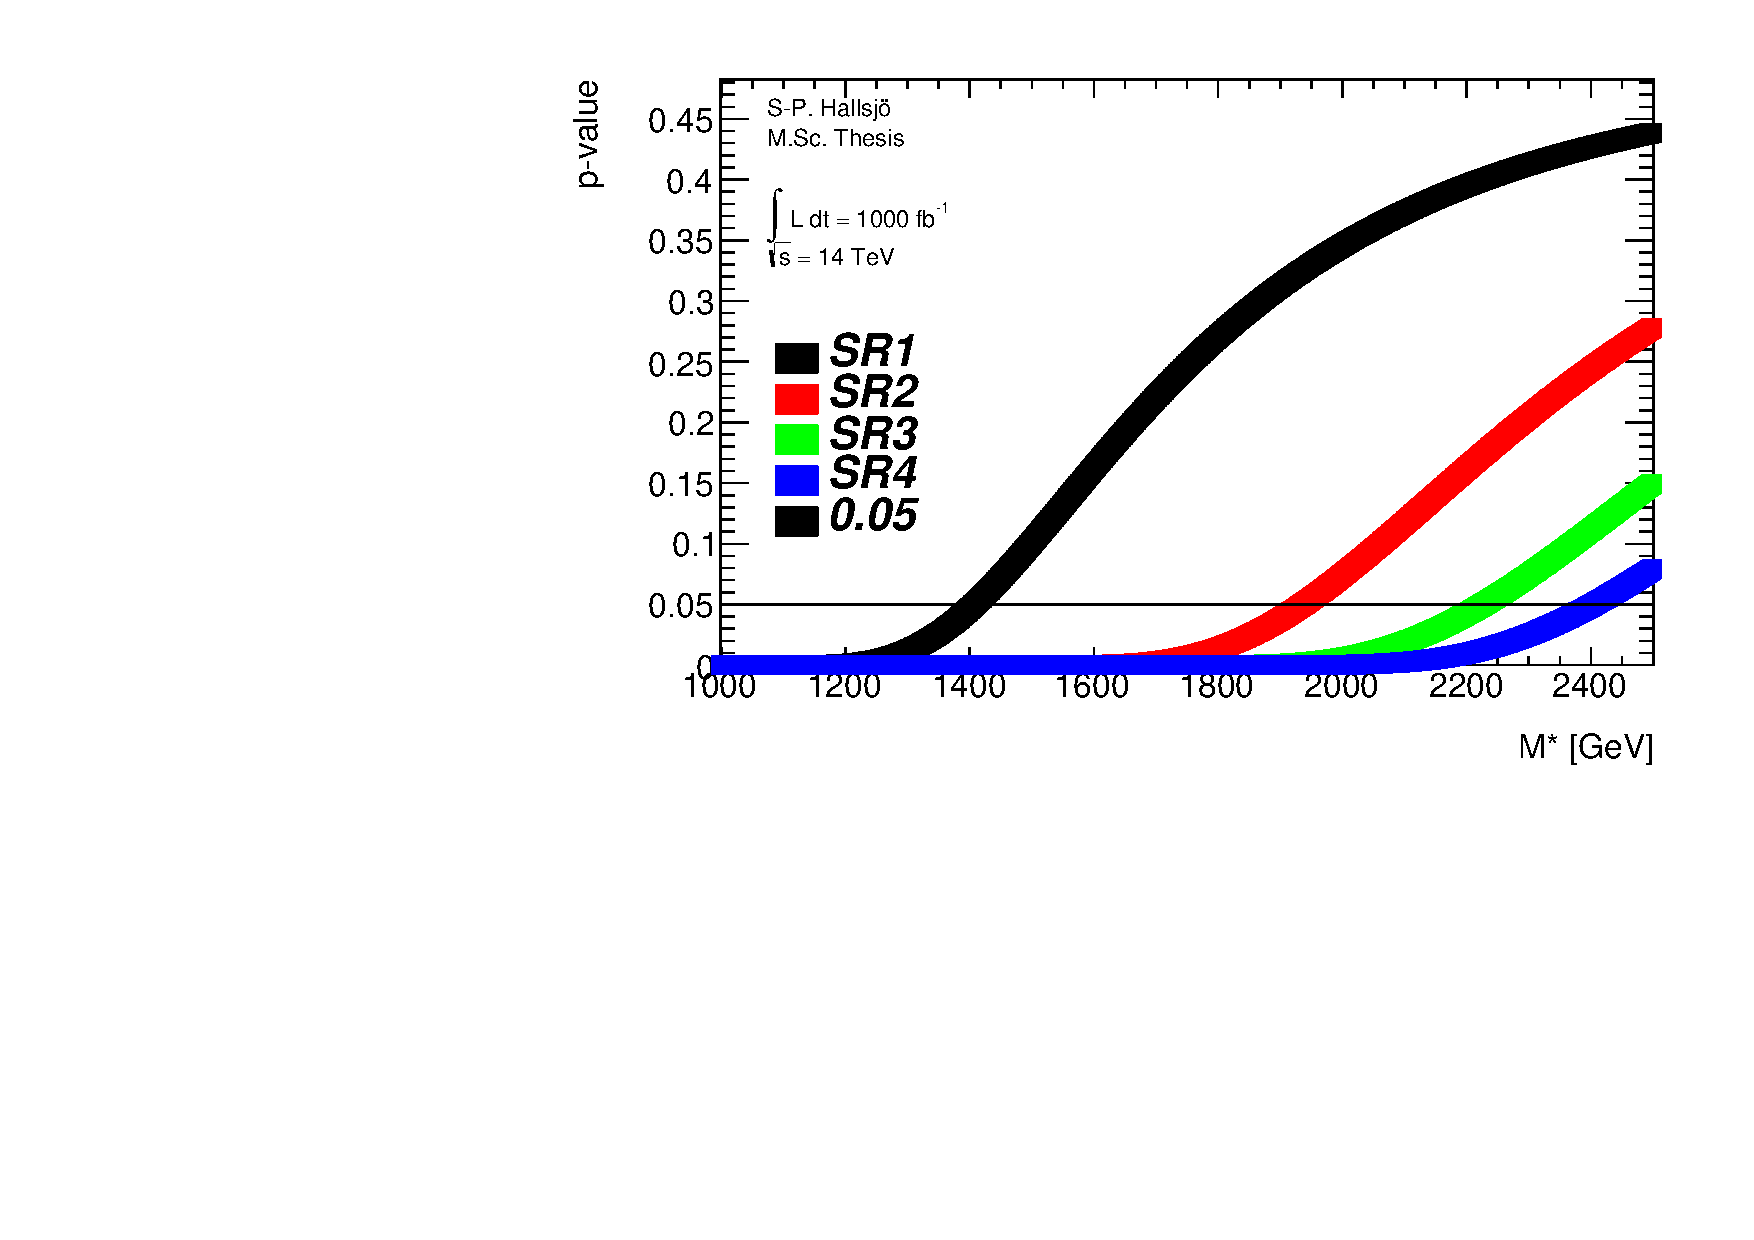
\includegraphics[width=0.5\textwidth]{pvald5002truth2.pdf}
    }
    \hfill
    \subfloat[ \label{fig:SRnewMt:2}]{%
      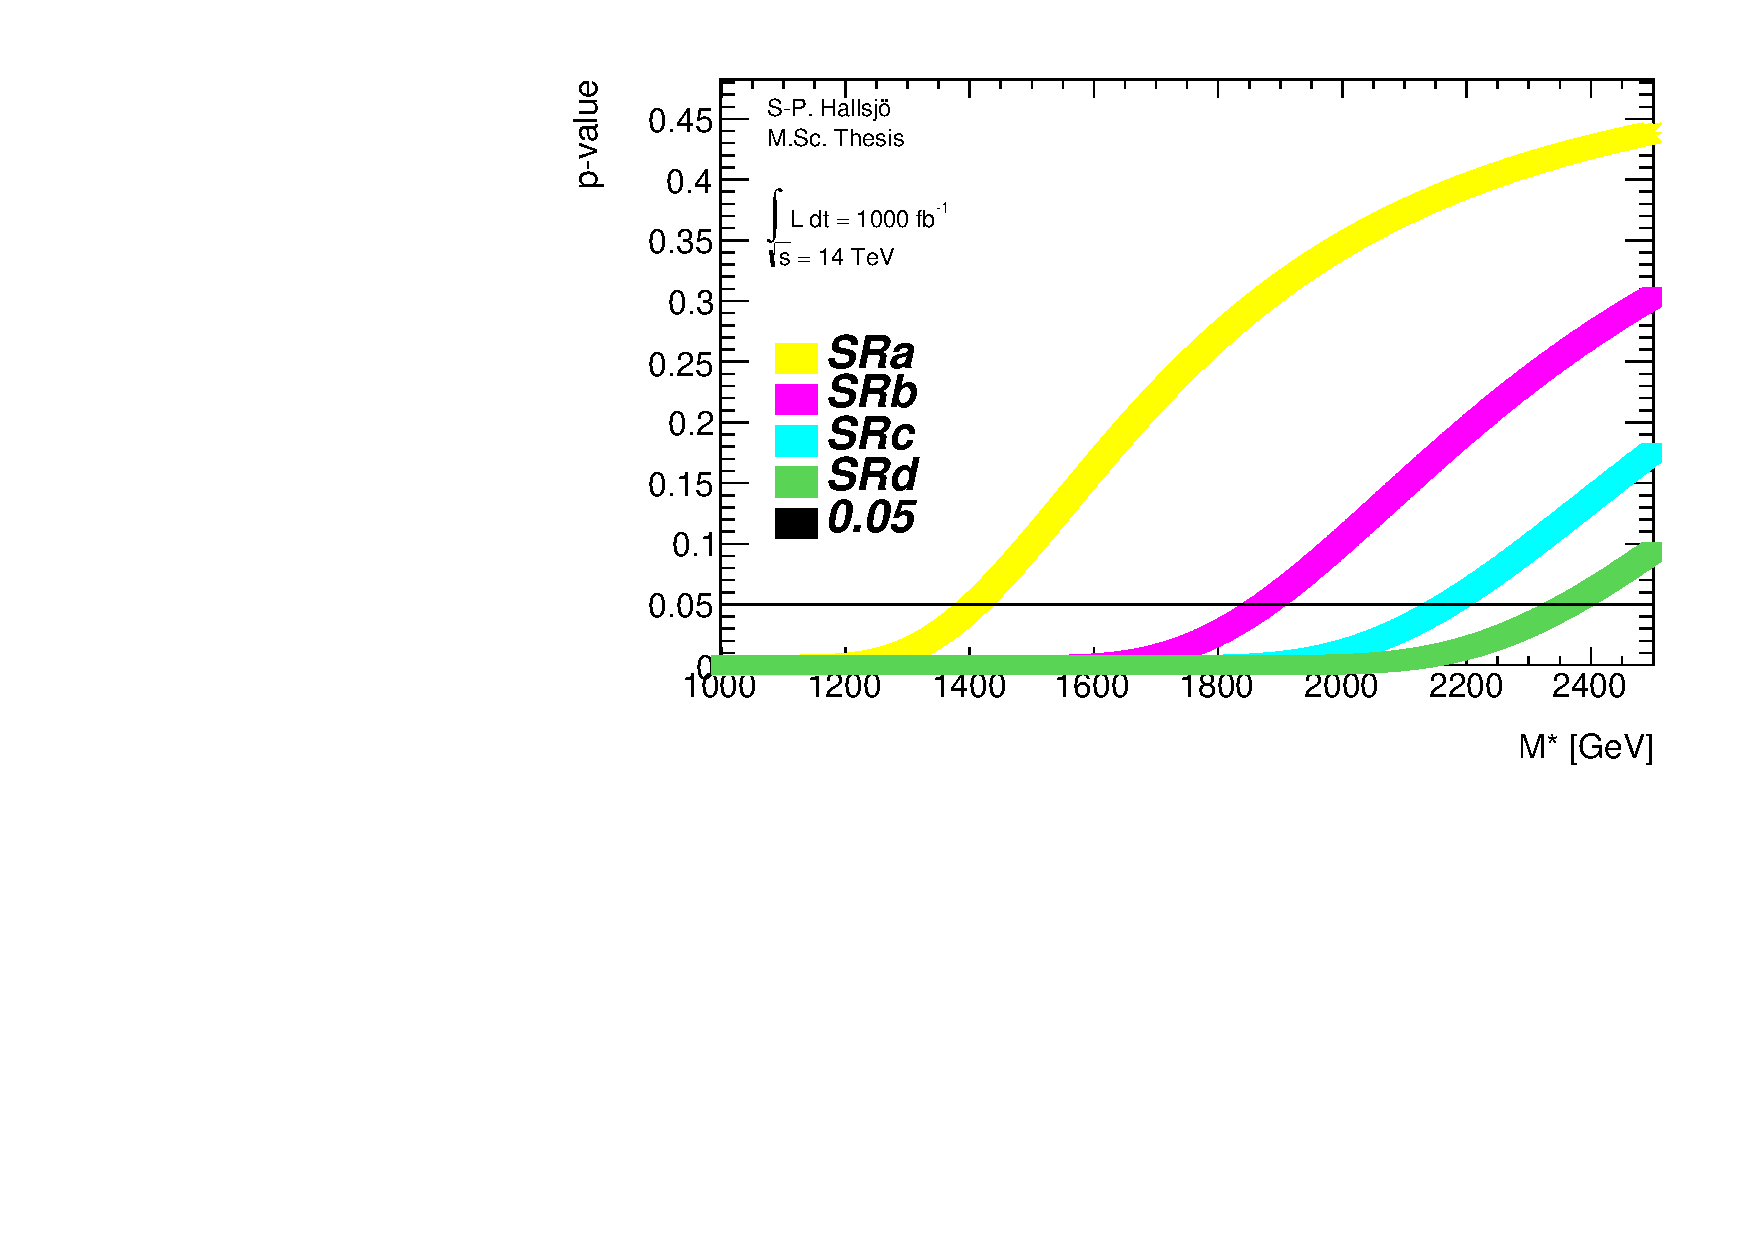
\includegraphics[width=0.5\textwidth]{pvald5002truth.pdf}
    }
    \caption{p-value as a function of the mass suppression scale M* at truth level for error model 0.02.}
    \label{fig:SRnewMt}
  \end{figure}
\newpage
 \begin{figure}[H] %!ht
    \subfloat[ \label{fig:SRnewMr:1}]{%
     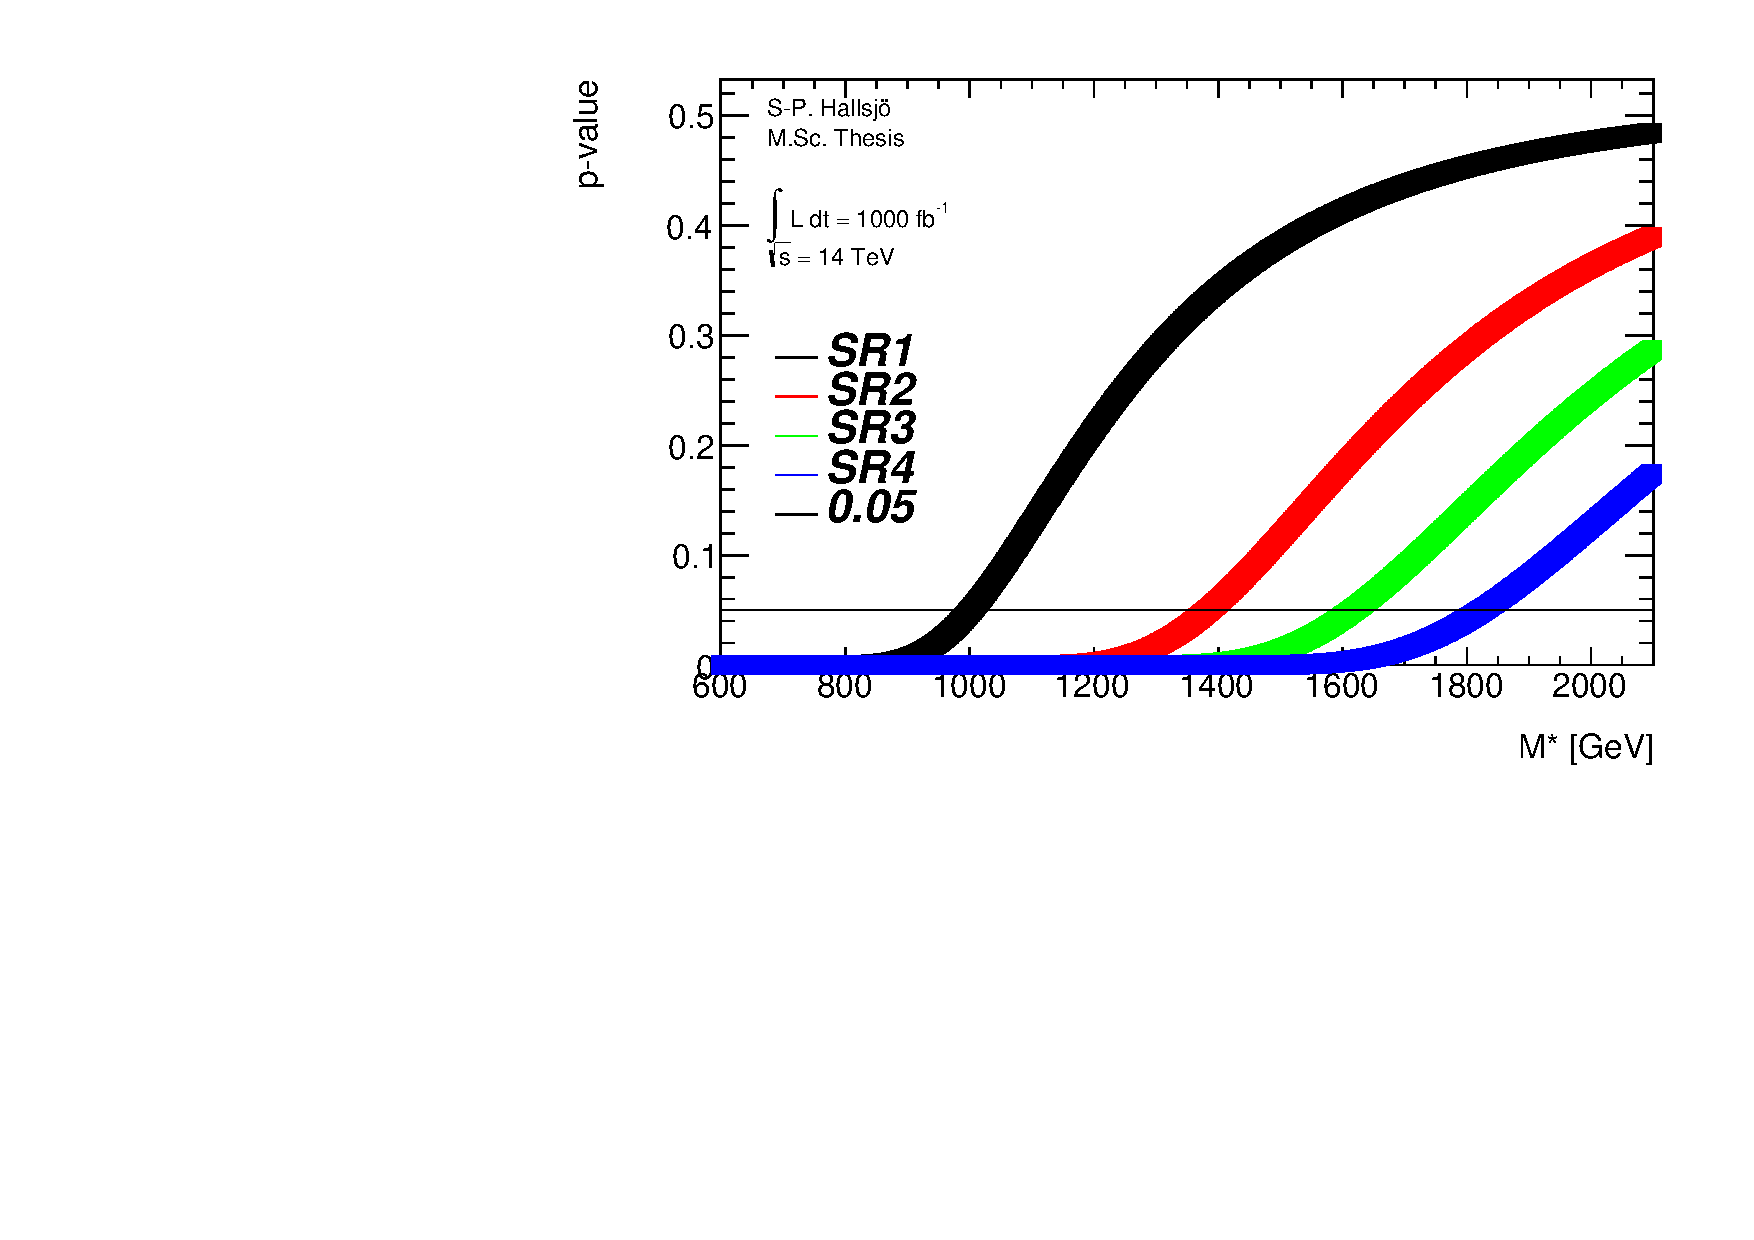
\includegraphics[width=0.5\textwidth]{pvald5008truth2.pdf}
    }
    \hfill
    \subfloat[ \label{fig:SRnewMr:2}]{%
      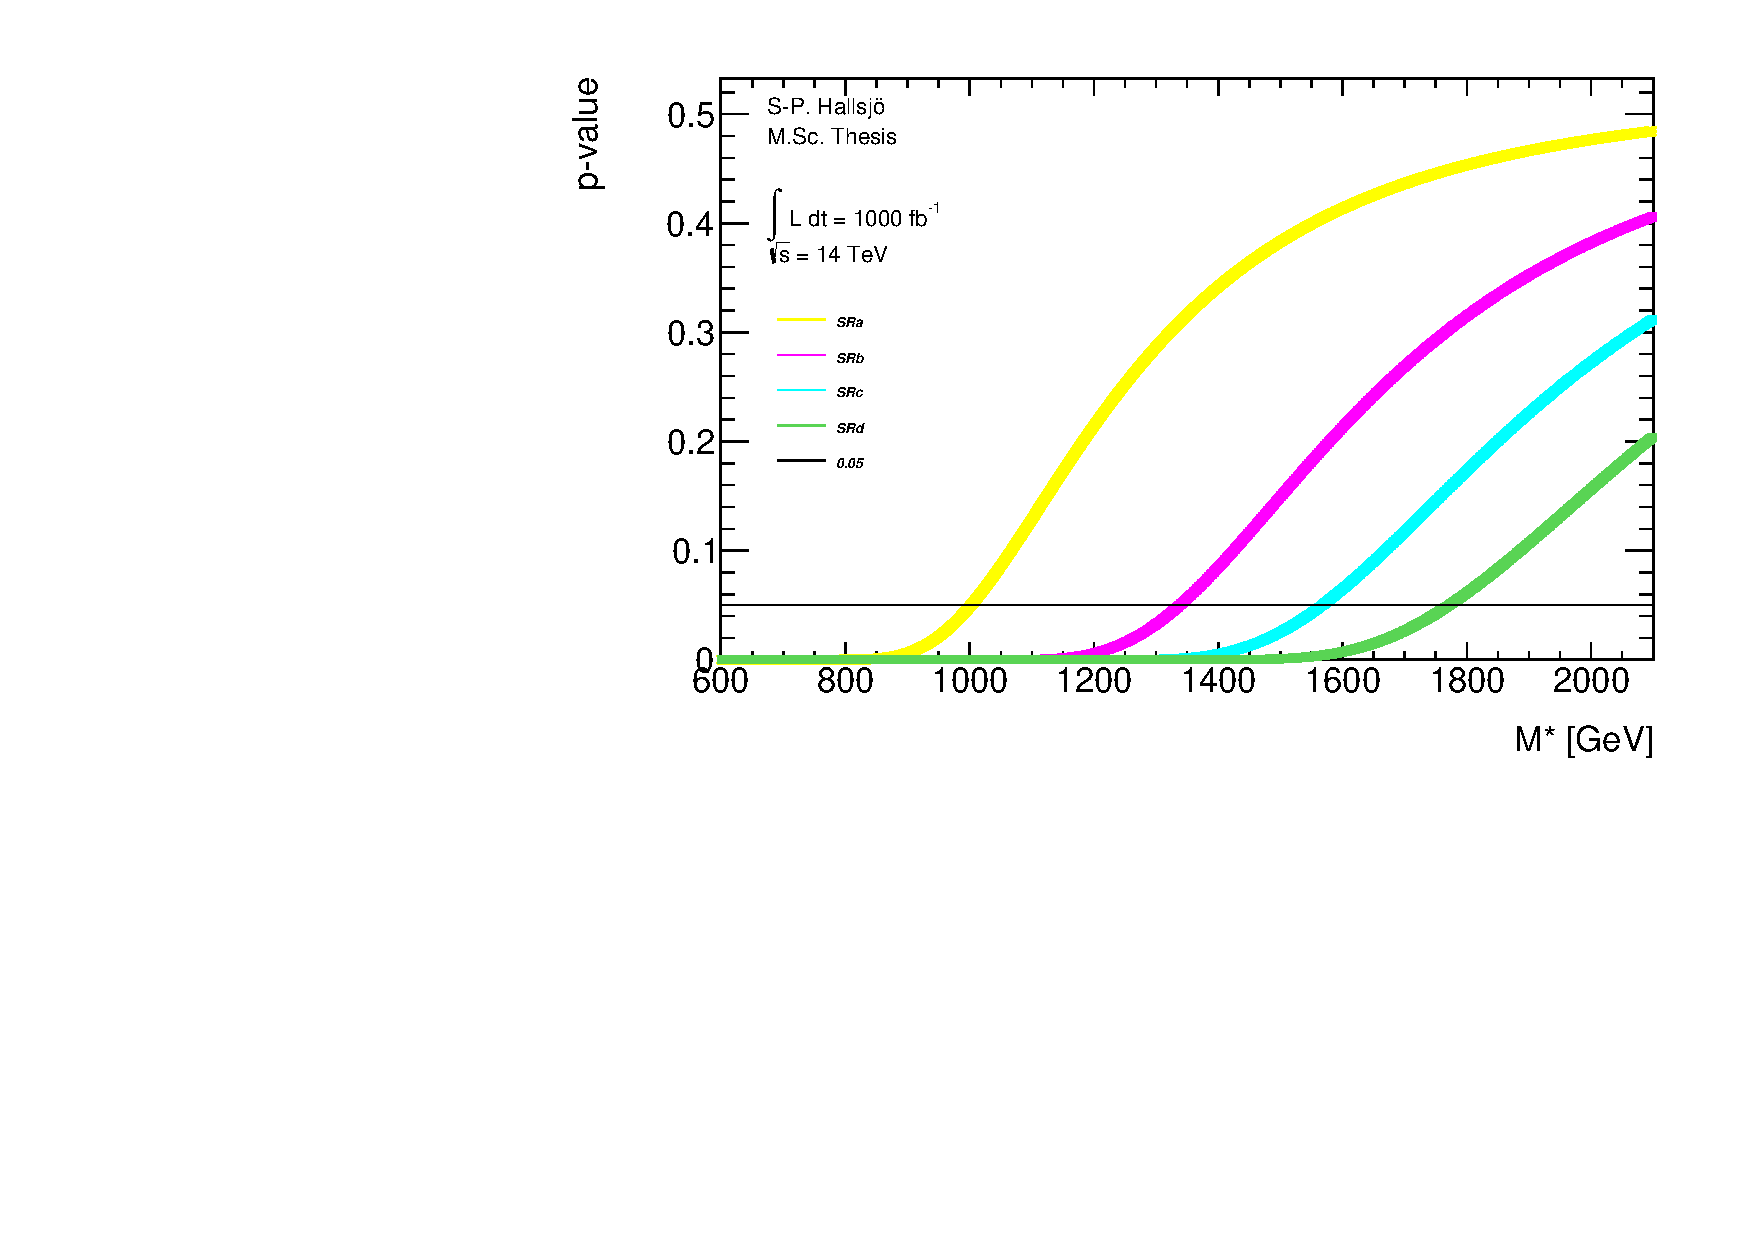
\includegraphics[width=0.5\textwidth]{pvald5008truth.pdf}
    }
    \caption{p-value as a function of the mass suppression scale M* at truth level for error model 0.08.}
    \label{fig:SRnewMr}
  \end{figure}

Calculating the intersection between these lines and 0.05 results in tables~\ref{tab:masssupp002}-~\ref{tab:masssupp2010} for both a dark matter mass of 50 GeV and at 400 GeV with the different error models.

\begin{table}[ht]
\begin{center}
\begin{tabular}{|l|l|l|}
\hline
Signal region & Truth [GeV]& Reconstructed [GeV]\\ \hline
SR1, symmetric 350 GeV &1407&1402\\
SR2, symmetric 600 GeV&1936&1934\\
SR3, symmetric 800 GeV&2227&2226\\
SR4, symmetric 1000 GeV&2404&2406\\ \hline
SRa, asymmetric 350 GeV &1425&1421\\
SRb, asymmetric 600 GeV &1874&1803\\
SRc, asymmetric 800 GeV&2169&2125\\
SRd, asymmetric 1000 GeV&2365&2340\\ \hline
\end{tabular}
\caption{Limits on mass suppression scales in GeV given for $m_{\chi}=50$ GeV and the 0.02 error model.}
\label{tab:masssupp002}
\end{center}
\end{table}

\begin{table}[ht]
\begin{center}
\begin{tabular}{|l|l|l|}
\hline
Signal region & Truth [GeV]& Reconstructed [GeV]\\ \hline
SR1, symmetric 350 GeV&1002&999\\
SR2, symmetric 600 GeV&1384&1382\\
SR3, symmetric 800 GeV&1617&1619\\
SR4, symmetric 1000 GeV&1825&1834\\ \hline
SRa, asymmetric 350 GeV&1338&1286\\
SRb, asymmetric 600 GeV&1356&1303\\
SRc, asymmetric 800 GeV&1567&1533\\
SRd, asymmetric 1000 GeV&1771&1745\\ \hline
\end{tabular}
\caption{Limits on mass suppression scales in GeV given for $m_{\chi}=50$ GeV and the 0.08 error model.}
\label{tab:masssupp010}
\end{center}
\end{table}

\begin{table}[ht!]
\begin{center}
\begin{tabular}{|l|l|l|}
\hline
Signal region & Truth [GeV]& Reconstructed [GeV]\\ \hline
SR1, symmetric 350 GeV &1333&1329\\
SR2, symmetric 600 GeV&1848&1847\\
SR3, symmetric 800 GeV&2162&2163\\
SR4, symmetric 1000 GeV&2332&2303\\ \hline
SRa, asymmetric 350 GeV&1350&1346\\
SRb, asymmetric 600 GeV&1789&1721\\
SRc, asymmetric 800 GeV&2106&2059\\
SRd, asymmetric 1000 GeV&2288&2258\\ \hline
\end{tabular}
\caption{Limits on mass suppression scales in GeV given for $m_{\chi}=400$ GeV and the 0.02 error model.}
\label{tab:masssupp2002}
\end{center}
\end{table}

\begin{table}[ht]
\begin{center}
\begin{tabular}{|l|l|l|}
\hline
Signal region & Truth [GeV]& Reconstructed [GeV]\\ \hline
SR1, symmetric 350 GeV&949&946\\
SR2, symmetric 600 GeV&1321&1320\\
SR3, symmetric 800 GeV&1570&1573\\
SR4, symmetric 1000 GeV&1770&1755\\ \hline

SRa, asymmetric 350 GeV&961&959\\
SRb, asymmetric 600 GeV&1277&1228\\
SRc, asymmetric 800 GeV&1521&1484\\
SRd, asymmetric 1000 GeV&1714&1684\\ \hline
\end{tabular}
\caption{Limits on mass suppression scales in GeV given for $m_{\chi}=400$ GeV and the 0.08 error model.}
\label{tab:masssupp2010}
\end{center}
\end{table}

Tables \ref{tab:masssupp002}-\ref{tab:masssupp2010} show the significant difference between the different signal regions, especially between SR4 and SRd which are similar apart from the lead jet momenta cut. Another interesting difference is how the limits are increased by using tighter signal regions. In these tables the effect from an increase in dark matter mass can be seen as small.

The effect of pile-up on $M$* can be seen by comparing the columns. The limits at reconstructed level can be better than at truth since the statistical approach by the smearing functions can either increase or decrease the number of events which are in a signal region. If the number of signal events is increased and the number of background events decreased the $M$* values will increase.

\subsection{Projection exclusion limits on mediator mass models}\label{sec:res:subsec:Mm}
For the vector mediator models described in \subsectionref{sec:signal:subsec:vecmed}, limits on which models can be excluded have been calculated. This is done by calculating which models have a $p$-value below 0.05. An example of an excludable and an unexcludable signal model can be seen in \figureref{fig:sigback}. The exclusion uses the two different error models, as described in \subsectionref{subsec:errdata}, when calculating the $p$-value. All signals which have been used can be found in \appendixref{livecmedpro}.

 \begin{figure}[H] %!ht
    \subfloat[An excludable signal model. \label{fig:sigback:1}]{%
     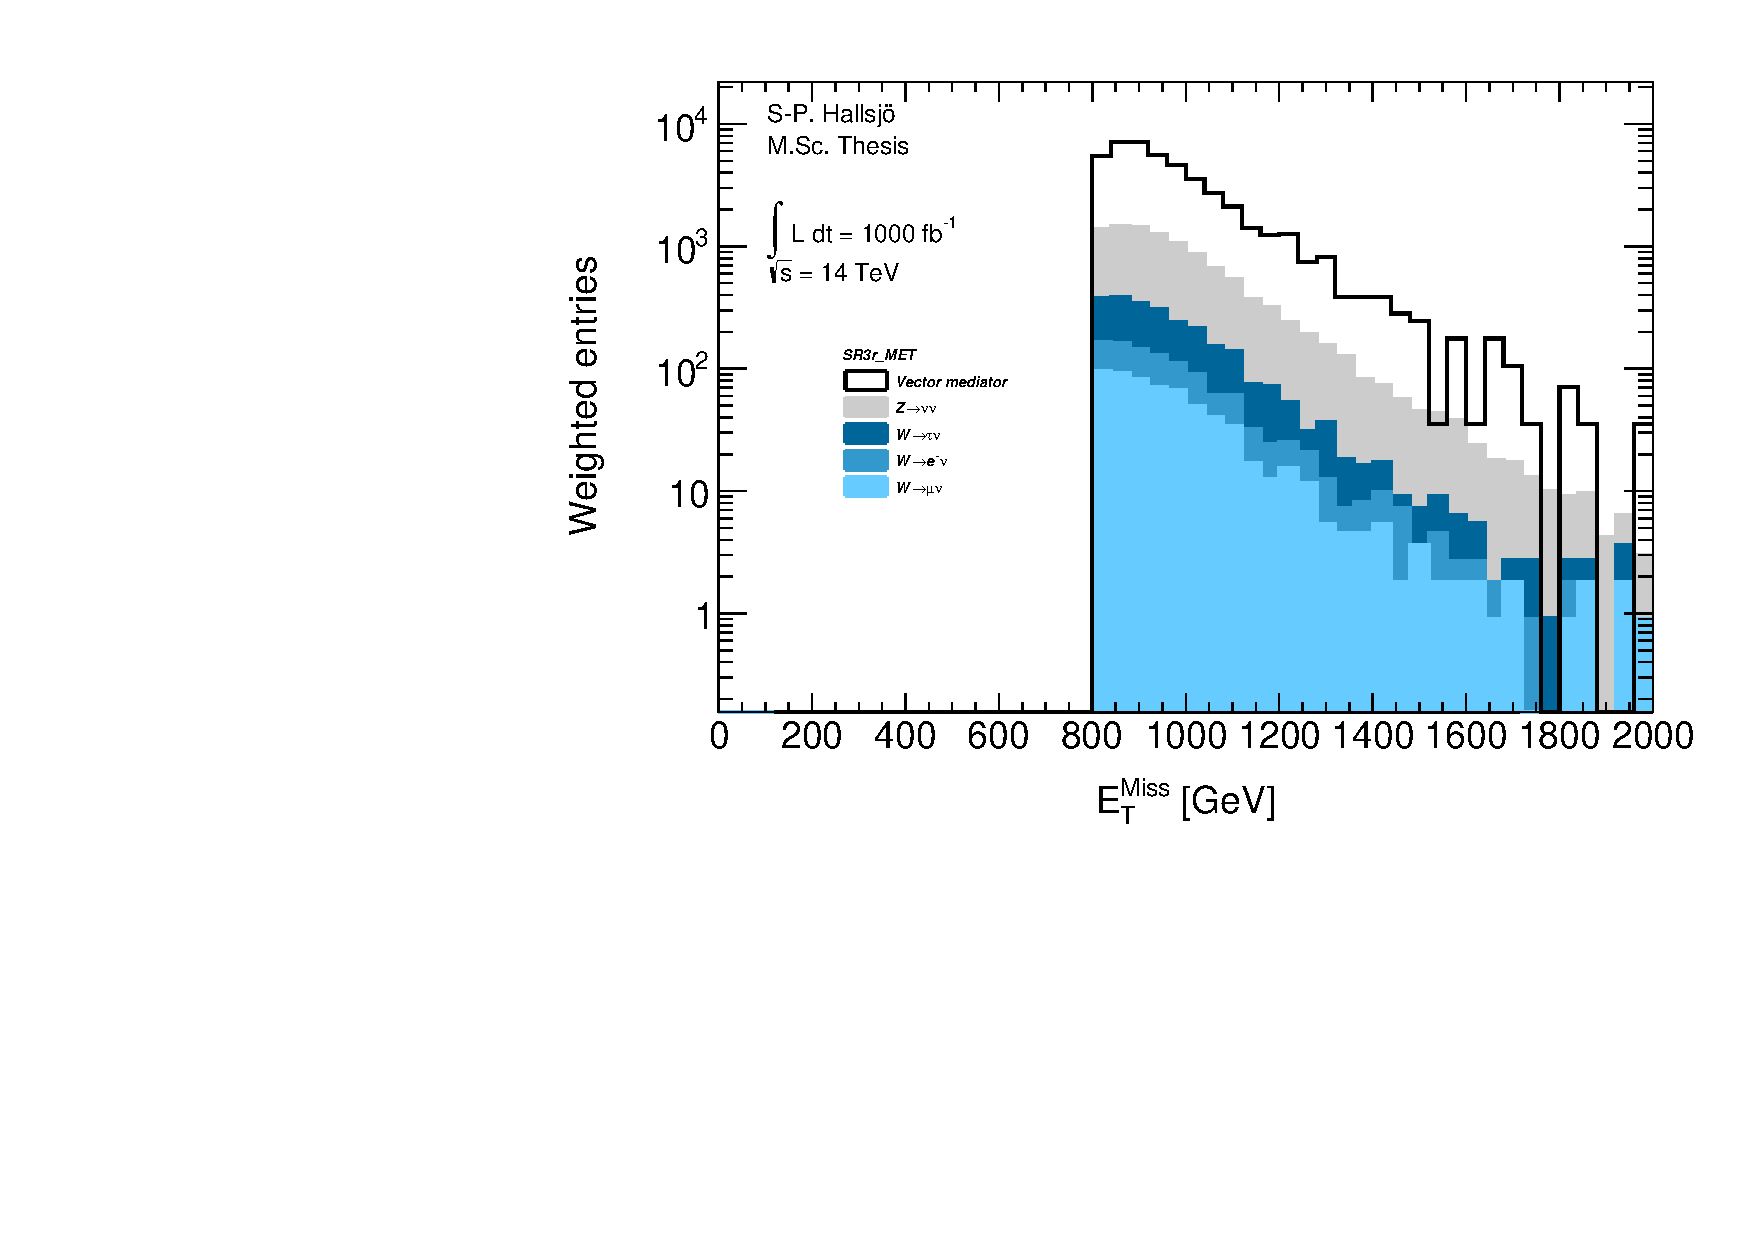
\includegraphics[width=0.5\textwidth]{mediator2.pdf}
    }
    \hfill
    \subfloat[A nonexcludable signal model. \label{fig:sigbacktau:2}]{%
      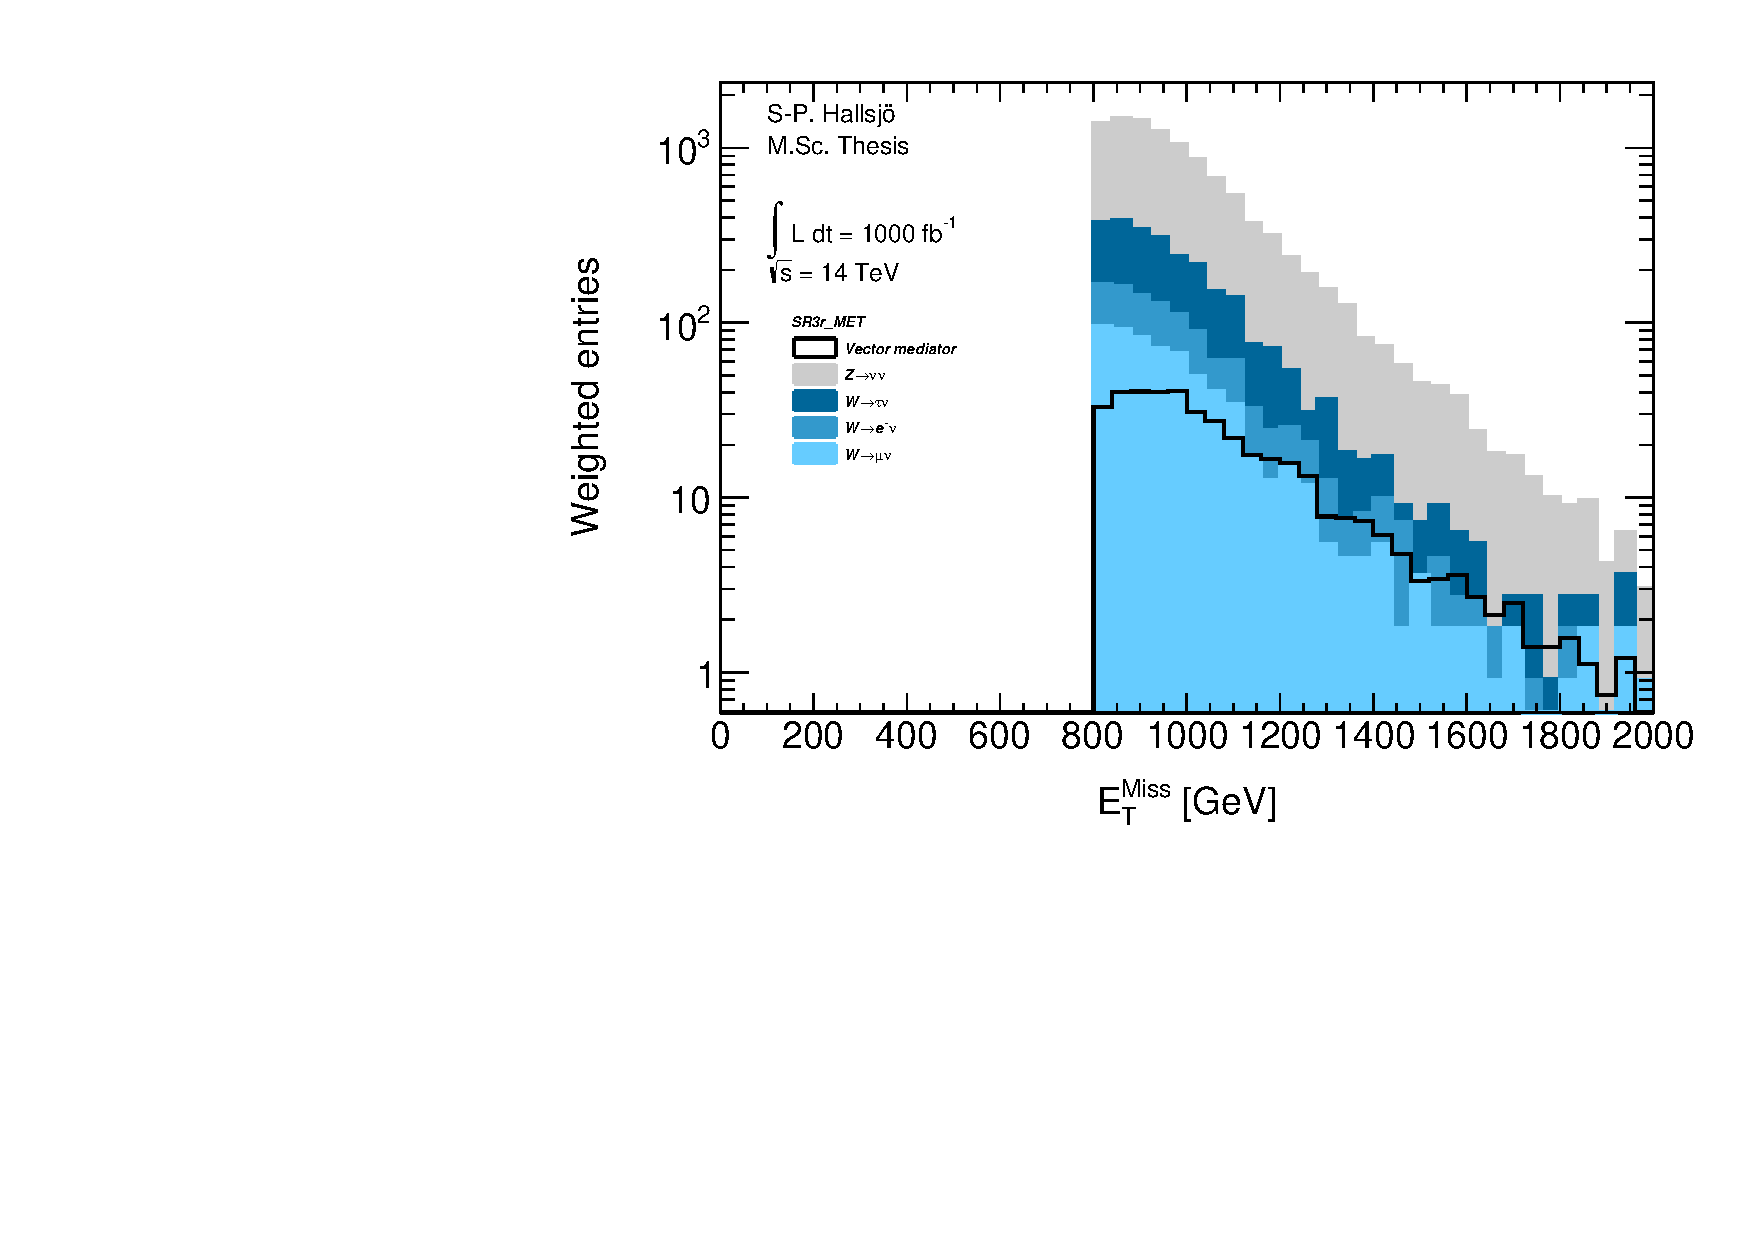
\includegraphics[width=0.5\textwidth]{mediator6.pdf}
    }
    \caption{Signal on background plot in log-scale for E$^{Miss}_T$ on a reconstructed level in SR3 to illustrate a signal which is excludable and one which is not. This is seen by the amount of signal compared to the amount of background.}
    \label{fig:sigback}
  \end{figure}

To set limits on the mediator mass models the $p$-value is calculated in different signal regions for the different signal models with different mediator mass. As an example, a plot of this in signal region SRd is given in \figureref{fig:modelex}, where the $p$-value of the models is plotted against the increasing mediator mass for different widths and dark matter masses. The result of which models are excludable, thus with a $p$-value $<0.05$, are given in tables \ref{tab:mediatorpass} and \ref{tab:mediatorpass2}.

 \begin{figure}[H] %!ht
    \subfloat[$p$-values at a reconstructed level for different mediator masses and dark matter masses at a width of m/3. \label{fig:modelex:1}]{%
     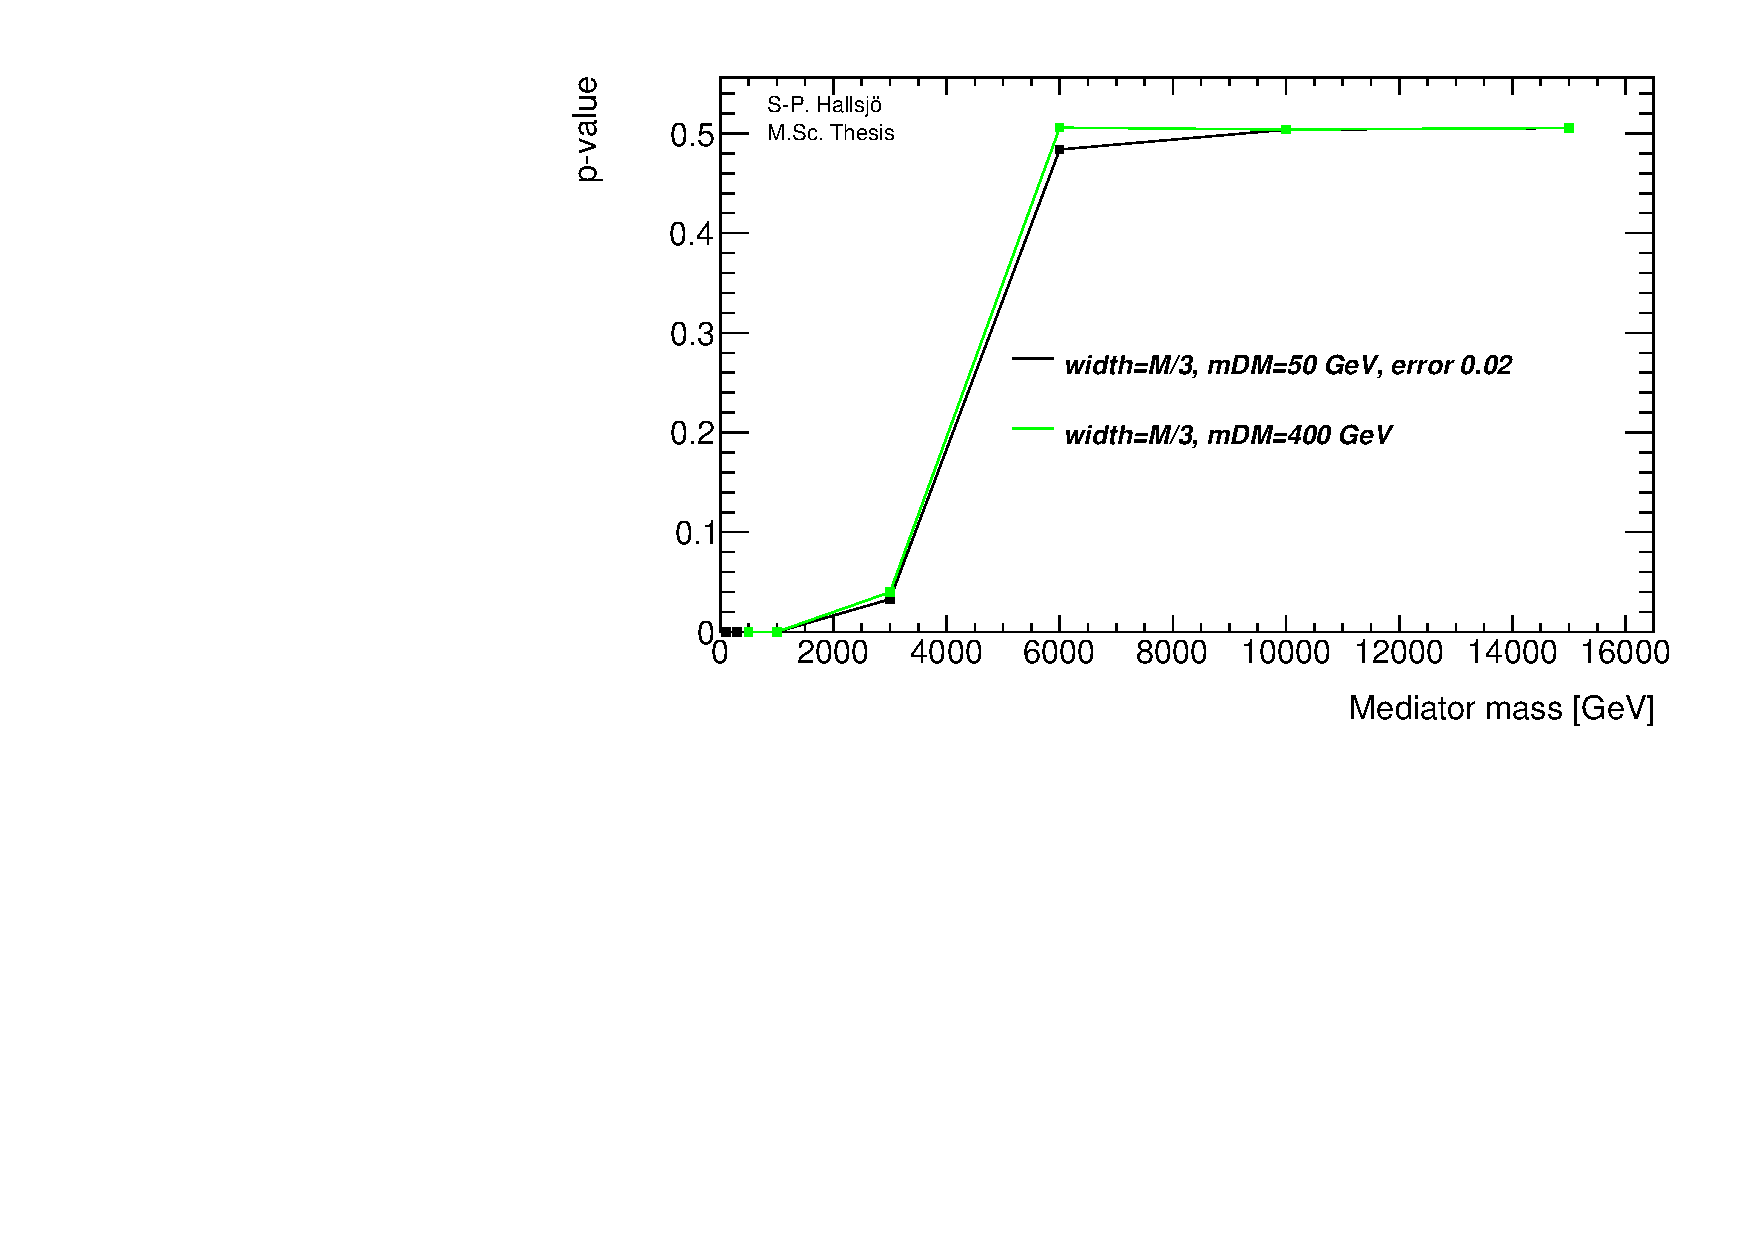
\includegraphics[width=0.5\textwidth]{reco3002.pdf}
    }
    \hfill
    \subfloat[$p$-values at a reconstructed level for different mediator masses and dark matter masses at a width of m/$8\pi$. \label{fig:modelex:2}]{%
      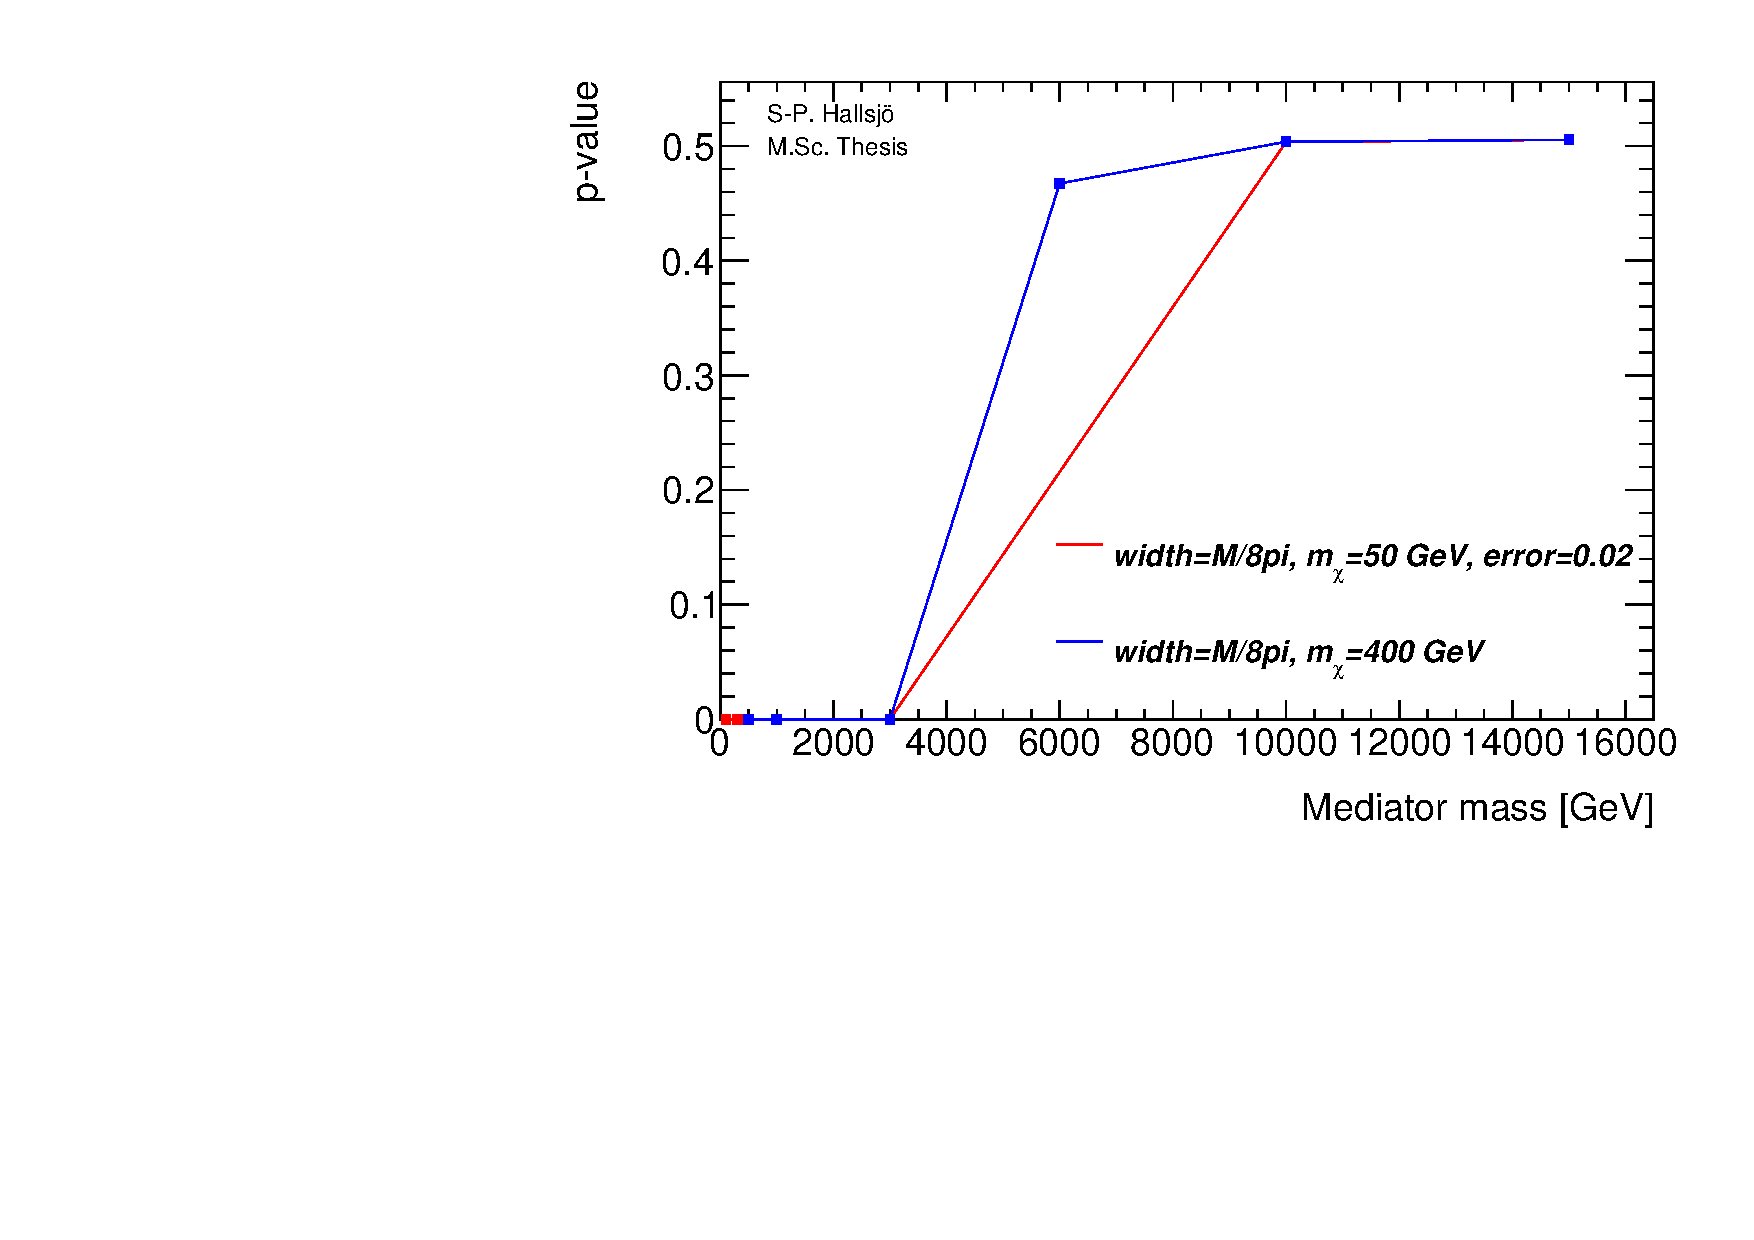
\includegraphics[width=0.5\textwidth]{reco8002.pdf}
    }
    \caption{$p$-values at a reconstructed level for the different mediator masses, dark matter masses and different widths which were investigated in SRd.}
    \label{fig:modelex}
  \end{figure}



\begin{table}[ht]
\begin{center}
\begin{tabular}{|l|l|l|}
\hline
width & $m_{\chi}=50$ GeV & $m_{\chi}=400$ GeV \\ \hline
M/3 & 1000 GeV & 1000 GeV \\ \hline
M/$8\pi$ & 3000 GeV & 3000 GeV\\ \hline
\end{tabular}
\caption{Limits on the highest mediator mass model which can be excluded for different widths, different dark matter masses for truth and reconstructed data and both error models in SR2, 3, 4, c, d.}
\label{tab:mediatorpass}
\end{center}
\end{table}
\begin{table}[ht]
\begin{center}
\begin{tabular}{|l|l|l|}
\hline
width & $m_{\chi}=50$ GeV & $m_{\chi}=400$ GeV \\ \hline
M/3 & 1000 GeV & 1000 GeV\\ \hline
M/$8\pi$ & 1000 GeV & 1000 GeV\\ \hline
\end{tabular}
\caption{Limits on the highest mediator mass model which can be excluded for different widths, different dark matter masses for truth and reconstructed data and both error models in SRb.}
\label{tab:mediatorpass2}
\end{center}
\end{table}

What can be seen in \tableref{tab:mediatorpass} and \tableref{tab:mediatorpass2} is that the models are robust since the limits are unchanged by a change in the error models and with the introduction of pile-up. However since there were no signal models available with mediator masses between 1000 and 3000 or between 3000 and 6000 no better limits can be set. These effects may be more visible when determining the mediator mass limit similar to the work done for $M$* and will also set the limits on the mediator mass. 

It is though quite interesting to see that SRb, compared to the other signal regions, is the signal region which was worst suited for the vector mediator signals. Looking at the definition of this signal region would suggest that the background is less susceptible to a lead jet cut than the signals.

\newpage
\section{Discussion}
\subsection{Comparison to previous results}
In \tableref{Comp pval} the limits for the mass suppression scale are given from both the paper and from this work. It is seen that the increase in luminosity and center of mass energy gives an increase of the mass suppression scale by a factor of 2-3.

\begin{table}[ht]
\begin{center}
\begin{tabular}{|l|l|l|}
\hline
Dark matter mass & From simulation & From paper \\ \hline
50 GeV & 1960 GeV &800 GeV \\
400 GeV & 1871 GeV & 700 GeV \\ \hline
\end{tabular}
\caption{M* values in SR2 from both simulation at 14 TeV, 1000fb$^{-1}$ and from Ref. \citep{ATLAS-CONF-2012-147} at 8 TeV and 10fb$^{-1}$. }
\label{Comp pval}
\end{center}
\end{table}

\subsection{Effect of the high luminosity}\label{subsec:hleff}
As seen in \sectionref{chap:sig:sec:res}, the effect of a pile-up rate of 140 is minute in the signal regions chosen. The primary focus of this thesis was to look at the effect of pile-up, and try to mitigate the effect of it. However, it is shown here that by choosing signal regions with a high enough requirement, the effect is minute. Thus the focus was shifted to perform a more in-depth mono-jet analysis of different dark matter signal models. 

For the mass suppression scale, as seen in \subsectionref{sec:res:subsec:m*}, comparing the truth values against the reconstructed values the difference is at most $<5 \% $. Thus, these signal regions are preferable for use in the high luminosity upgrade. 

Regarding the mediator models, as discussed in \subsectionref{sec:res:subsec:Mm} the models are sensitive to exclusion regardless of truth or reconstructed data. By investigating more models, the limits on the mediator masses can be set and the effects of pile-up seen more clearly.

\newpage
\section{Conclusion}
\subsection{Limit on M*}
The limits can be found in \subsectionref{sec:res:subsec:m*} and are 2-3 times better than previous results at 8 TeV and 10fb$^{-1}$.

\subsection{Limit on mediator mass models}
The limits are found in \subsectionref{sec:res:subsec:Mm} and is the first result done with these models and thus can not be compared.

\subsection{Effect of the high luminosity}
At a pile-up level of 140 the effect is at most $<5\%$ compared to truth level on the mass suppression scale and does not affect the vector mediator models which are robust as discussed in \subsectionref{subsec:hleff}.